% Template file for an a0 landscape poster.
% Written by Graeme, 2001-03 based on Norman's original microlensing
% poster.
%
% See discussion and documentation at
% <http://www.astro.gla.ac.uk/users/norman/docs/posters/> 
%
% $Id: poster-template-landscape.tex,v 1.2 2002/12/03 11:25:46 norman Exp $


% Default mode is landscape, which is what we want, however dvips and
% a0poster do not quite do the right thing, so we end up with text in
% landscape style (wide and short) down a portrait page (narrow and
% long). Printing this onto the a0 printer chops the right hand edge.
% However, 'psnup' can save the day, reorienting the text so that the
% poster prints lengthways down an a0 portrait bounding box.
%
% 'psnup -w85cm -h119cm -f poster_from_dvips.ps poster_in_landscape.ps'

\documentclass[a0]{a0poster}
% You might find the 'draft' option to a0 poster useful if you have
% lots of graphics, because they can take some time to process and
% display. (\documentclass[a0,draft]{a0poster})
\input defs
\pagestyle{empty}
\setcounter{secnumdepth}{0}
\renewcommand{\familydefault}{\sfdefault}
\newcommand{\QED}{~~\rule[-1pt]{8pt}{8pt}}\def\qed{\QED}


%\usepackage[T1, T2A]{fontenc}			% Пакет выбора кодировки и шрифтов
%\usepackage[utf8]{inputenc} 			% любая желаемая кодировка
%\usepackage[english]{babel}		% поддержка русского языка
%\usepackage{wrapfig}					% Плавающие картинки
\usepackage{amssymb, amsmath}			% стилевой пакет для формул
\usepackage{algorithm}
\usepackage{algorithmic} 
%\usepackage{natbib}
\usepackage{mathptmx}

\usepackage[pdftex]{graphicx}
\usepackage{pgfplotstable}

\renewcommand{\reals}{{\mbox{\bf R}}}

% The textpos package is necessary to position textblocks at arbitary 
% places on the page.
\usepackage[absolute]{textpos}

\usepackage{fleqn,psfrag,wrapfig,tikz}

\usepackage[papersize={38in,28in}]{geometry}

% Graphics to include graphics. Times is nice on posters, but you
% might want to switch it off and go for CMR fonts.
\usepackage{graphics}
\usepackage{hyperref}

% we are running pdflatex, so convert .eps files to .pdf
%\usepackage[pdftex]{graphicx}
%\usepackage{epstopdf}

% These colours are tried and tested for titles and headers. Don't
% over use color!
\usepackage{color}
\definecolor{Red}{rgb}{0.9,0.0,0.1}

\definecolor{bluegray}{rgb}{0.15,0.20,0.40}
\definecolor{bluegraylight}{rgb}{0.35,0.40,0.60}
\definecolor{gray}{rgb}{0.3,0.3,0.3}
\definecolor{lightgray}{rgb}{0.7,0.7,0.7}
\definecolor{darkblue}{rgb}{0.2,0.2,1.0}
\definecolor{darkgreen}{rgb}{0.0,0.5,0.3}

\renewcommand{\labelitemi}{\textcolor{bluegray}\textbullet}
\renewcommand{\labelitemii}{\textcolor{bluegray}{--}}

\setlength{\labelsep}{0.5em}
\usepackage{subcaption}

% see documentation for a0poster class for the size options here
\let\Textsize\normalsize
%\def\Head#1{\noindent\hbox to \hsize{\hfil{\LARGE\color{bluegray} #1}}\bigskip}
\def\Head#1{\noindent{\LARGE\color{bluegray} #1}\bigskip}
\def\LHead#1{\noindent{\LARGE\color{bluegray} #1}\bigskip}
\def\Subhead#1{\noindent{\large\color{bluegray} #1}\bigskip}
\def\Title#1{\noindent{\VeryHuge\color{Red} #1}}


% Set up the grid
%
% Note that [40mm,40mm] is the margin round the edge of the page --
% it is _not_ the grid size. That is always defined as 
% PAGE_WIDTH/HGRID and PAGE_HEIGHT/VGRID. In this case we use
% 23 x 12. This gives us three columns of width 7 boxes, with a gap of
% width 1 in between them. 12 vertical boxes is a good number to work
% with.
%
% Note however that texblocks can be positioned fractionally as well,
% so really any convenient grid size can be used.
%
\TPGrid[40mm,40mm]{23}{12}      % 3 cols of width 7, plus 2 gaps width 1

\parindent=0pt
\parskip=0.2\baselineskip

\begin{document}

% Understanding textblocks is the key to being able to do a poster in
% LaTeX. In
%
%    \begin{textblock}{wid}(x,y)
%    ...
%    \end{textblock}
%
% the first argument gives the block width in units of the grid
% cells specified above in \TPGrid; the second gives the (x,y)
% position on the grid, with the y axis pointing down.

% You will have to do a lot of previewing to get everything in the 
% right place.

% This gives good title positioning for a portrait poster.
% Watch out for hyphenation in titles - LaTeX will do it
% but it looks awful.
\begin{textblock}{23}(0,0)
\Title{Stochastic Universal Gradient}
\end{textblock}

\begin{textblock}{23}(0,0.6)
{
\LARGE
Evgenii Lagutin
}

{
\Large
\color{bluegray}
\emph{Optimization Class Project. MIPT}
}
\end{textblock}


% Uni logo in the top right corner. A&A in the bottom left. Gives a
% good visual balance, but you may want to change this depending upon
% the graphics that are in your poster.
%\begin{textblock}{2}(0,10)
%Your logo here
%%\includegraphics{/usr/local/share/images/AandA.epsf}
%\end{textblock}

%\begin{textblock}{2}(21.2,0)
%Another logo here
%%\resizebox{2\TPHorizModule}{!}{\includegraphics{/usr/local/share/images/GUVIu/GUVIu.eps}}
%\end{textblock}


\begin{textblock}{7.0}(0,1.5)

\hrule\medskip
\Head{Introduction}\\
The universal gradient method is known to be a good approach to numerical optimization when one doesn't have information about the Lipsitz constant of the gradient. This adaptive method adjusts $L$ at each step of the optimization process and holds the following estimation of the number of calls to the oracle, returning the gradient of the minimized function:
\begin{center}$N=\underset{\nu\in[0,1]}{inf}\left(\dfrac{2L_{\nu}R^{1+\nu}}{\varepsilon}\right)^{\dfrac{2}{1+\nu}},$\end{center}
$$ \|\nabla f(x)-\nabla f(y)\|_2\le L_{\nu}\|y-x\|_2^{\nu}, \nu \in [0,1],~L_0 < \infty$$
But this estimation hasn't been transferred on the stochastic case. The purpose of the project is to investigate the effectiveness of the stochastic universal gradient method in practice. 

\medskip
\hrule\medskip
\Head{Algorithm}\\
{\Large{Adaptive Stochastic Gradient \\(Spokoiny's practical variant)}}

%\begin{algorithm}[h!]	
    \hspace*{\algorithmicindent} \textbf{Input}: lower estimate for the variance of the gradient $D_0 \le D$,\\ accuracy $0 < \varepsilon< \frac{D_0}{L}$, starting point $x_0 \in Q$, initial guess $L_{-1} > 0$
	\label{RKalg}
	\begin{algorithmic}[1] 
		\FOR {$k=0,1,...$}
		\STATE Set $i_k=0$. Set $r^k = \lceil \frac{2 D_0}{L_{k-1}} {\varepsilon}\rceil$, generate i.i.d. $\xi^i_K, ~i = 1,\dots, r^k$
		\REPEAT
		\STATE Set $L_k = 2 ^{i_k-1}L_{k-1}$
		\\
		\STATE Calculate $\tilde{g}(x_k) = \frac{1}{r^k}\sum_{i=1}^{r^k}\nabla f(x_k, \xi^i_k)$.
		\\
		\STATE Calculate $w_k = x_k - \frac{1}{2 L_k}\tilde{g}(x_k)$.
		\\
		\STATE Calculate $\tilde{f}(x_k) = \frac{1}{r_k}\sum_{i=1}^{r^k}f(x_k, \xi^i_k)$ and\\ $\tilde{f}(w_k) = \frac{1}{r^k}\sum_{i=1}^{r^k}f(w_k, \xi^i_k)$.
		\\
		\STATE Set $i_k = i_k + 1$.
		\UNTIL \\$~~~~\tilde{f}(w_k) \le \tilde{f}(x_k) + \langle\tilde{g}(x_k), w_k - x_k\rangle + \frac{2 L_k}{2}\|w_k - x_k\|_2^2 + \frac{\varepsilon}{10}$.
		\STATE Set $x_{k+1} = w_k,~k=k+1$.
		\ENDFOR
	\end{algorithmic}
%\end{algorithm}

\medskip
\hrule\medskip
\Head{Optimization of deep neural networks}\\
Let $g(x)$ be a stochastic gradient of the function being minimized.

In every iteration we have to check if the following inequality is satisfied:

\begin{center}$f(w) \le f(x) + \langle g(x), w-x \rangle + \frac{2L}{2}\|w-x\|^2_2 + \frac{\varepsilon}{10}$\end{center}

Substituting $w$ with the its definition expression, $w = x - \frac{1}{2L}g(x)$

We will get $f(w) \le f(x) - \frac{1}{2L}\|g(x)\|^2_2 + \frac{2L}{2}\frac{1}{4L^2}\|g(x)\|^2_2 + \frac{\varepsilon}{10}$\\ or $f(w) \le f(x) - \frac{1}{4L}\|g(x)\|^2_2 +  \frac{\varepsilon}{10}$


Consider f(x) to be a function of a range of matrices and vectors: 

\begin{center}$f(x)  = f(W_1, b_1, \dots, W_n, b_n),$\end{center}

\begin{center}$df(W_1,b_1,\dots,W_n, b_n) = \sum\limits_{i=1}^n(\dfrac{\partial f}{\partial W_i}dW_i+ \dfrac{\partial f}{\partial b_i}db_i)(W_1,b_1,\dots,W_n,b_n)$\end{center}

\end{textblock}

\begin{textblock}{7.0}(8,1.5)
	
The goal is to represent $df$ in this fashion:

\begin{center}$df(x) = \langle g(x), dx \rangle$\end{center}

In this case $g(x)$ is the gradient.

Let's notice that in case of $x$ is vector, $x \in \mathbb R^n, ~g(x) \in \mathbb R^n$

\begin{center}$\langle g(x), x\rangle = \sum\limits_{i=1}^n g_i(x) x_i $\end{center}

and so we do if $X$ is a matrix: $X \in Mat(n\times m), ~g(X) \in Mat(n\times m)$

\begin{center}$\langle g(X), X \rangle = \mathbf{tr}g(X)X = g(X) \cdot X = \sum_{i=1}^n\sum_{j=1}^mg_{ij}(X)X_{ij}$\end{center}

That means we may consider $X$ as a vector $(x_{11},x_{12},\dots,x_{1m},x_{21},\dots,x_{nm})$ of dimension $nm$ and the result will not change.

Such reasoning  allows us to compute the second norm of the gradient in a following way:

$\|g(x)\|_2^2 = \|g(W_1,b_1,\dots,W_n,b_n)\|_2^2 = \sum\limits_{i=1}^n \left(g_{W_1}(x)\cdot g_{W_1}(x) + \langle g_{b_1}(x)  , g_{b_1}(x)\rangle\right)$


\medskip
\hrule\medskip
\Head{Numerical Experiments}\\
\Subhead{Linear Regression}

\begin{minipage}{0.5\textwidth}
	\begin{center}
		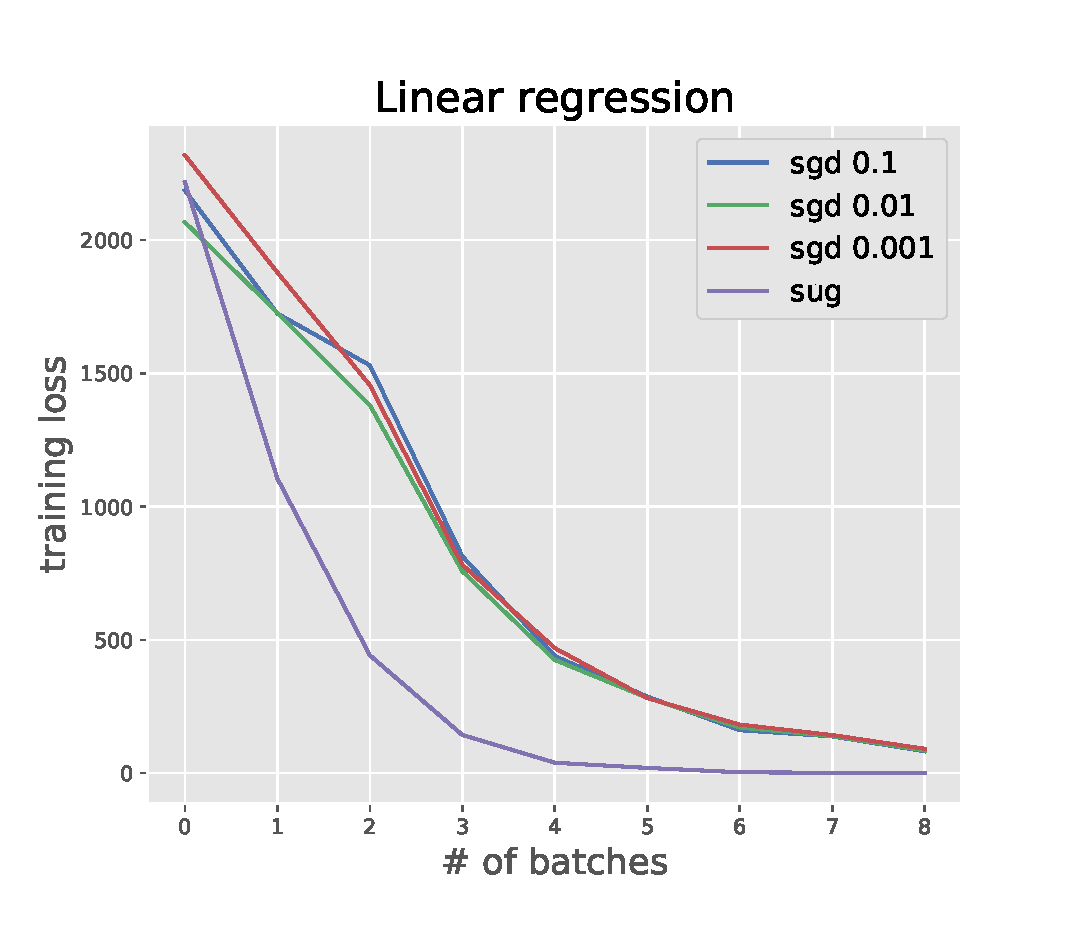
\includegraphics[width=1\textwidth]{figures/linreg.eps}
	\end{center}
\end{minipage}
\begin{minipage}{0.5\textwidth}
	\begin{center}
		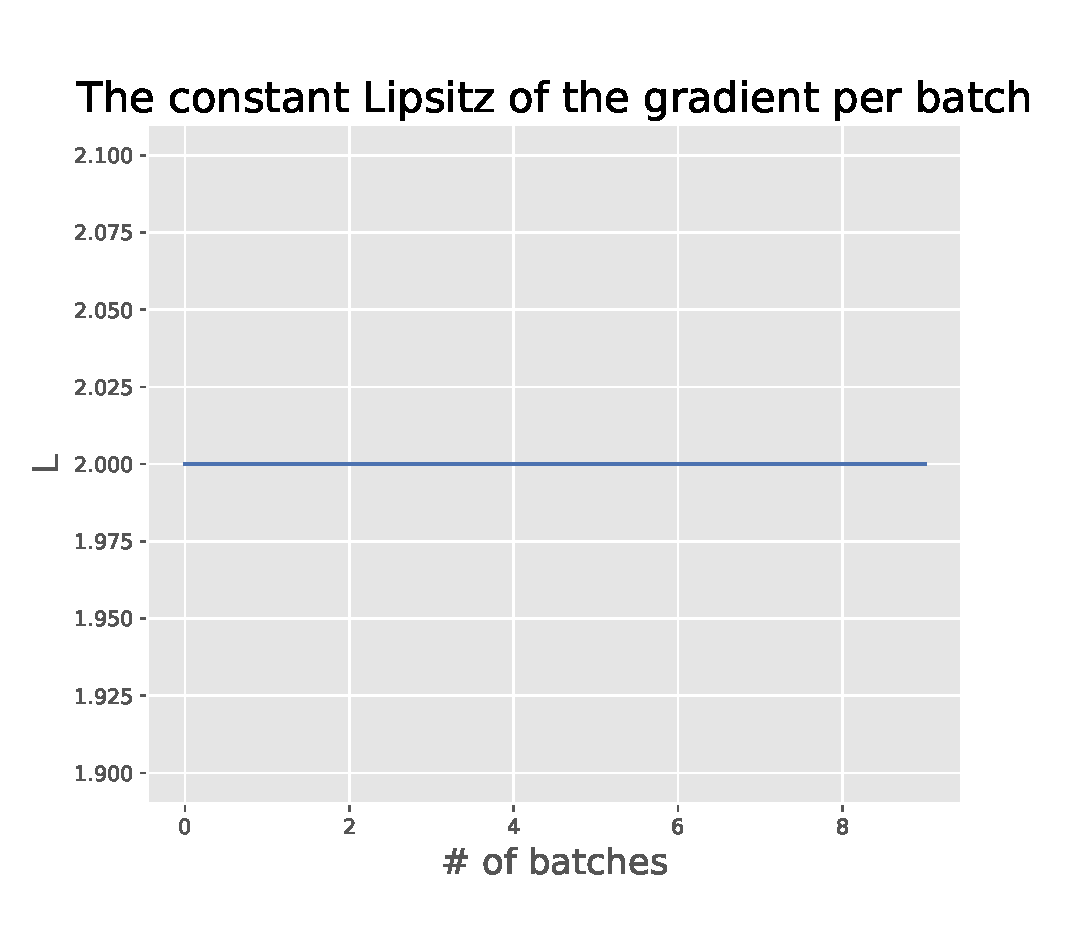
\includegraphics[width=1\textwidth]{figures/linreg_L.eps}
	\end{center}
\end{minipage}
\Subhead{MNIST}

\begin{minipage}{0.5\textwidth}
	\begin{center}
		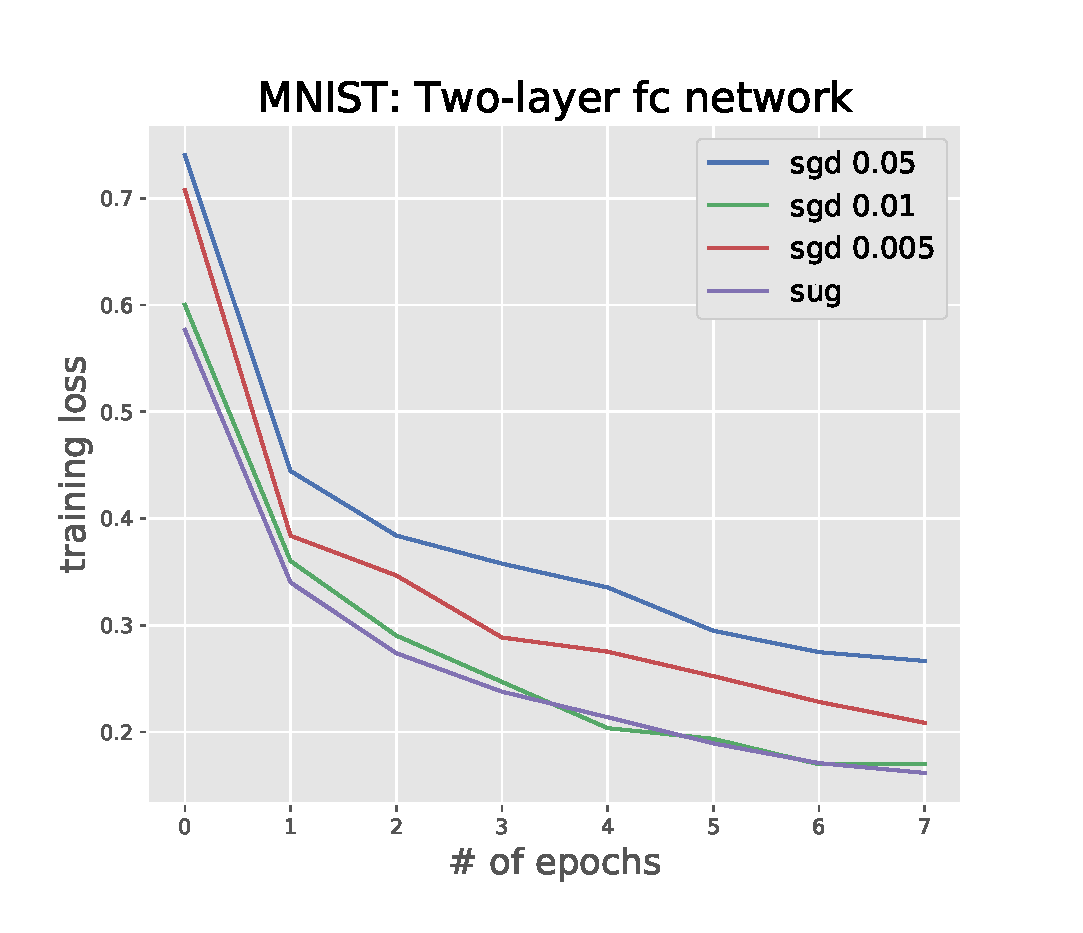
\includegraphics[width=1\textwidth]{figures/mnist_fc_ep.eps}
	\end{center}
\end{minipage}
\begin{minipage}{0.5\textwidth}
	\begin{center}
		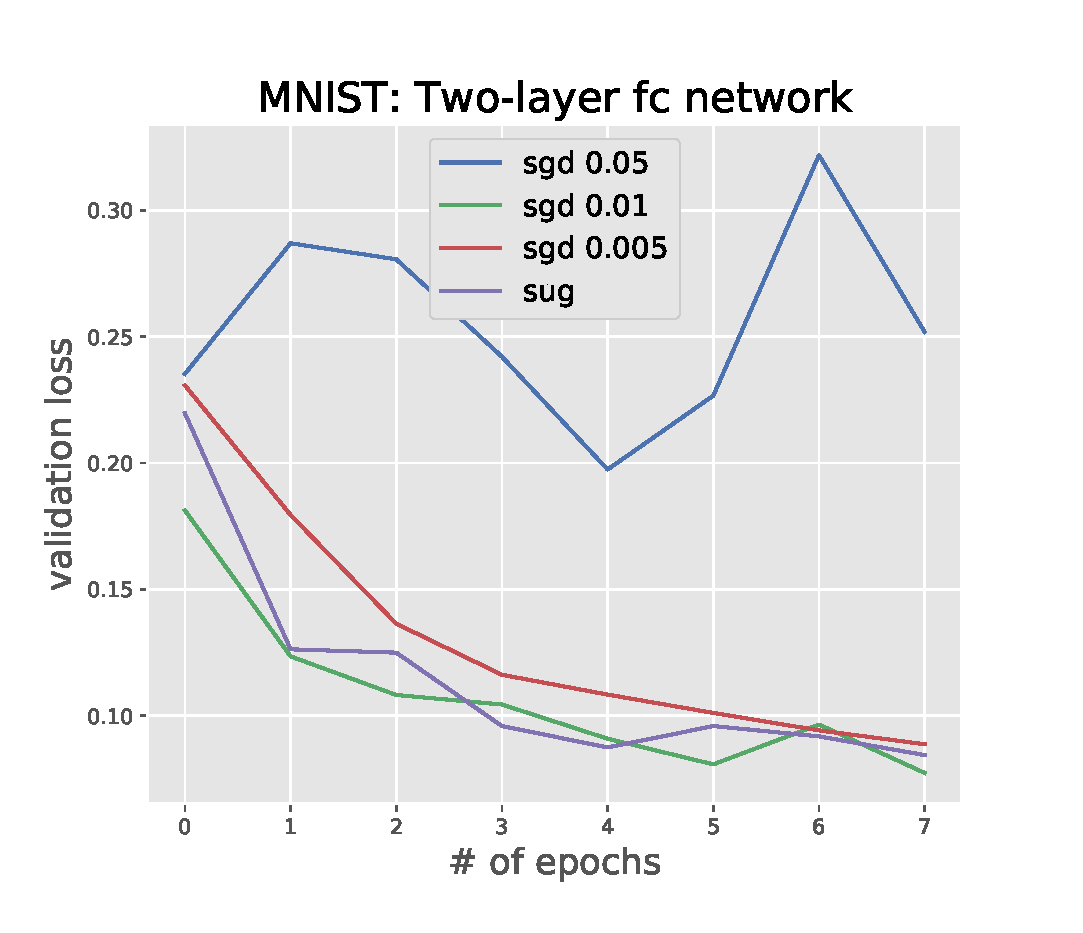
\includegraphics[width=1\textwidth]{figures/mnist_fc_val.eps}
	\end{center}
\end{minipage}
\begin{center}
	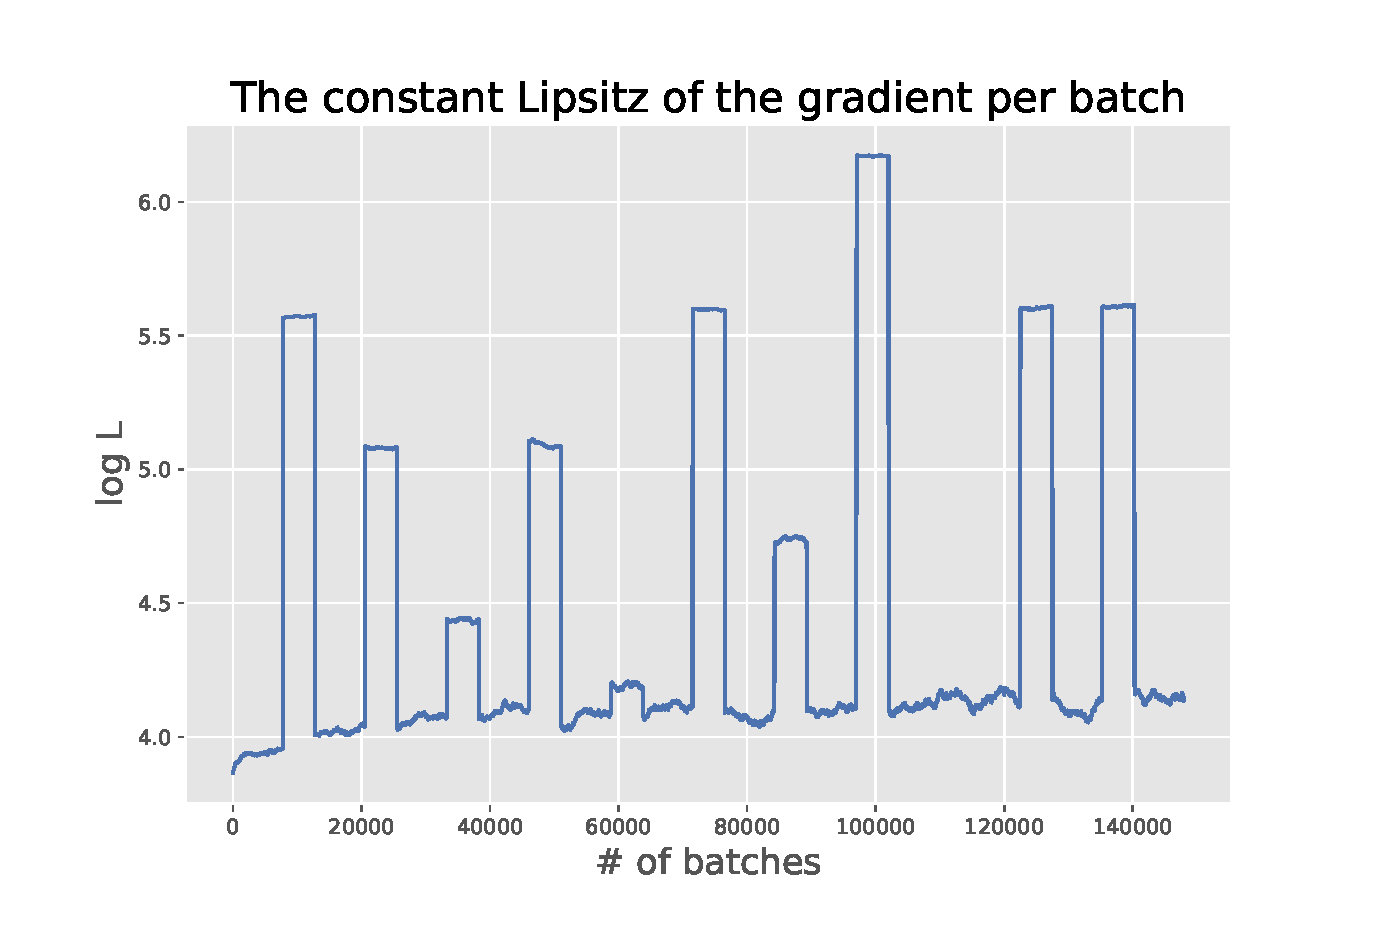
\includegraphics[width=0.53\textwidth]{figures/mnist_fc_L.eps}
\end{center}

\end{textblock}

\begin{textblock}{7.0}(16,1.5)
\Subhead{CIFAR10}

\begin{minipage}{0.5\textwidth}
	\begin{center}
		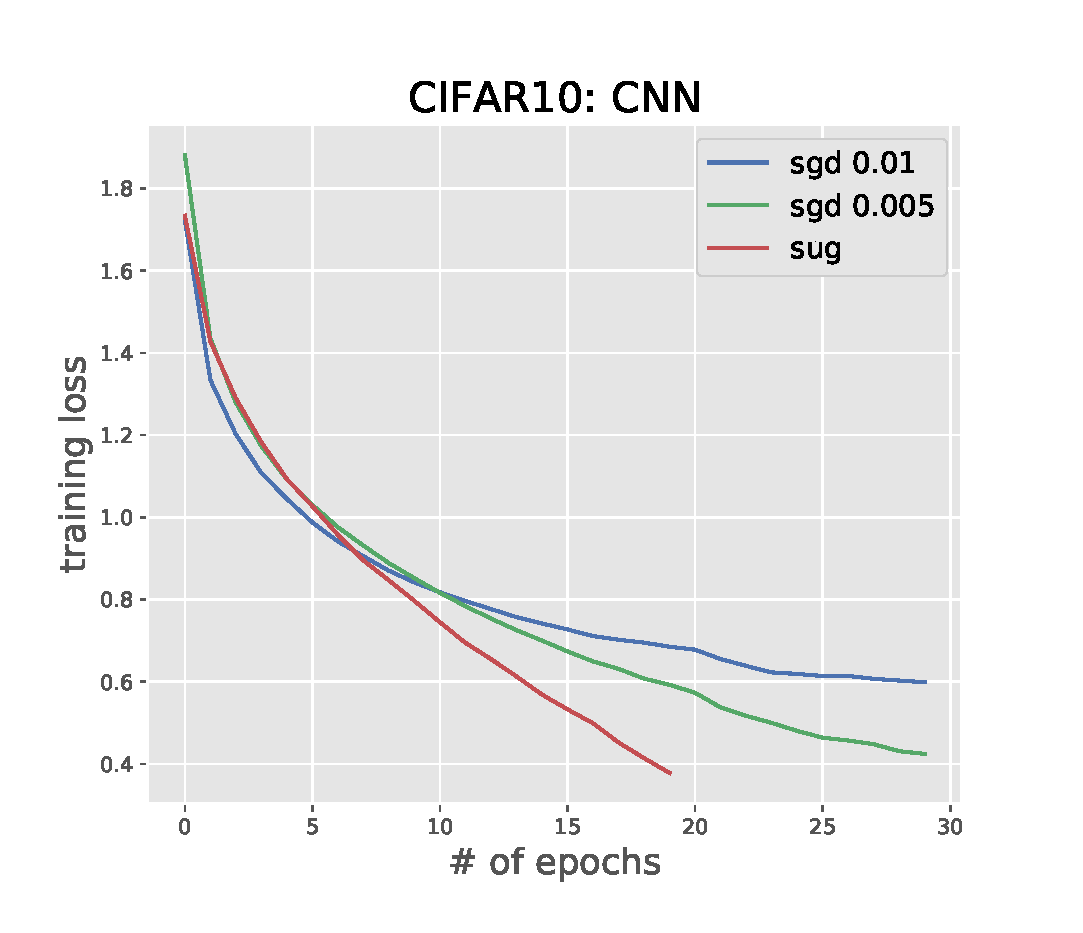
\includegraphics[width=1\textwidth]{figures/cifar_cnn_ep.eps}
	\end{center}
\end{minipage}
\begin{minipage}{0.5\textwidth}
	\begin{center}
		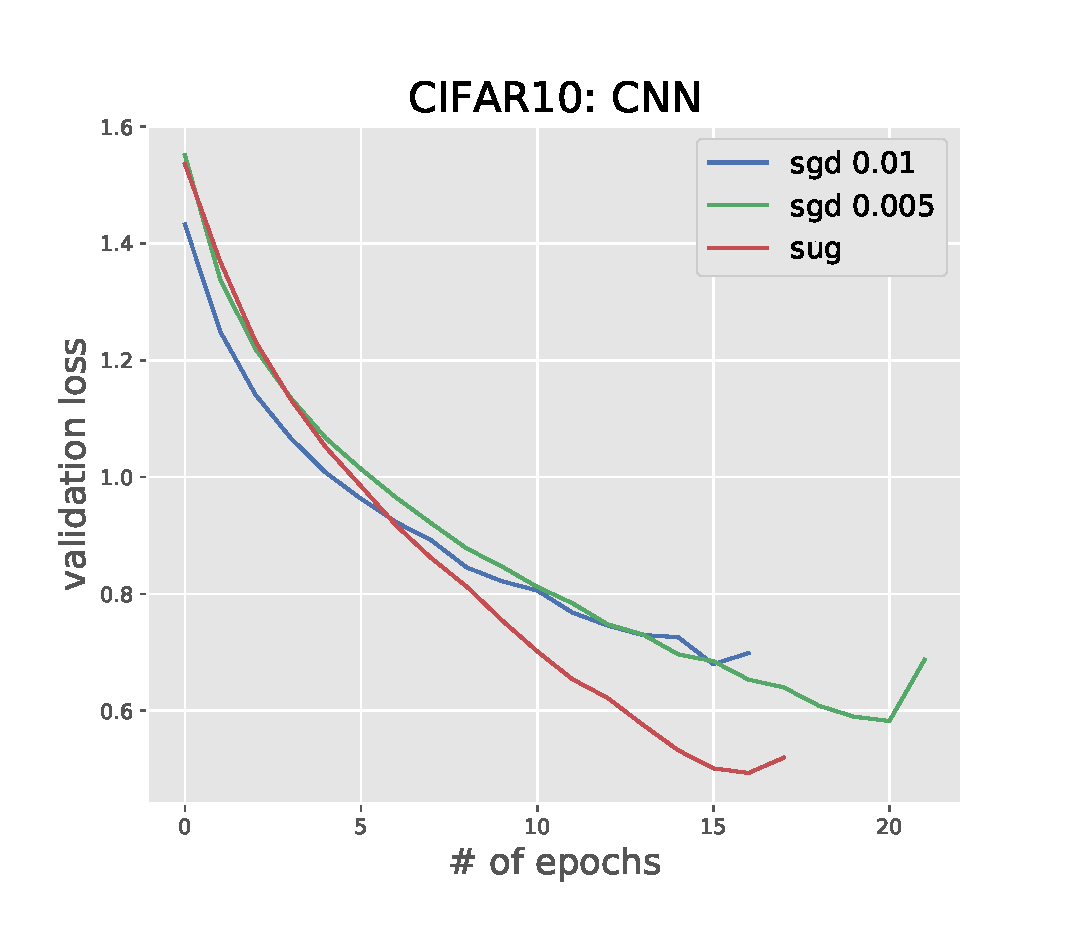
\includegraphics[width=1\textwidth]{figures/cifar_cnn_val.eps}
	\end{center}
\end{minipage}
\begin{center}
	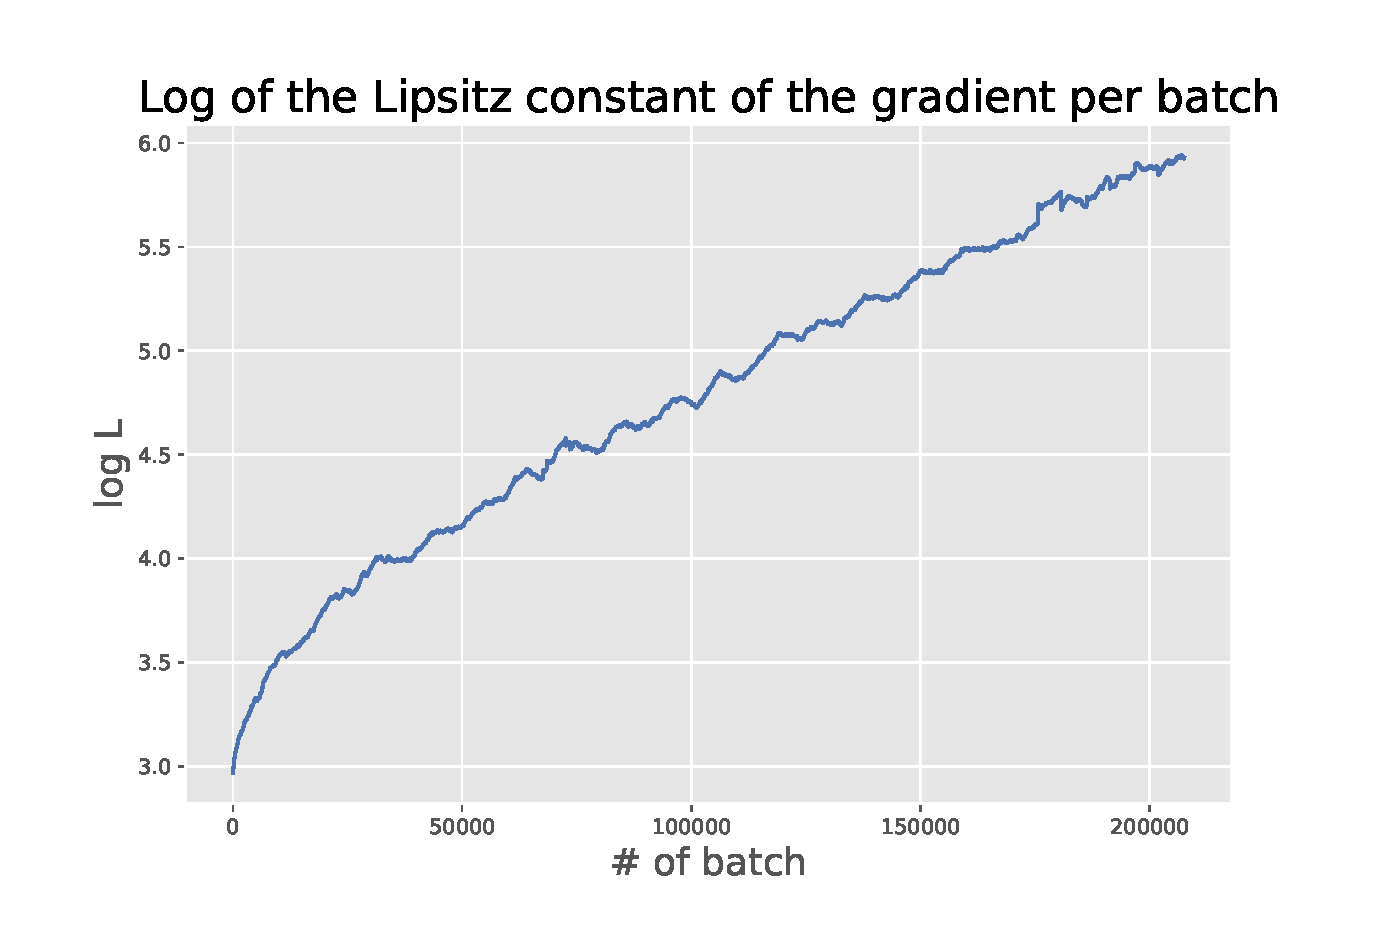
\includegraphics[width=0.6\textwidth]{figures/cifar_cnn_L.eps}
\end{center}

\Subhead{IMDb}

\begin{minipage}{0.5\textwidth}
	\begin{center}
		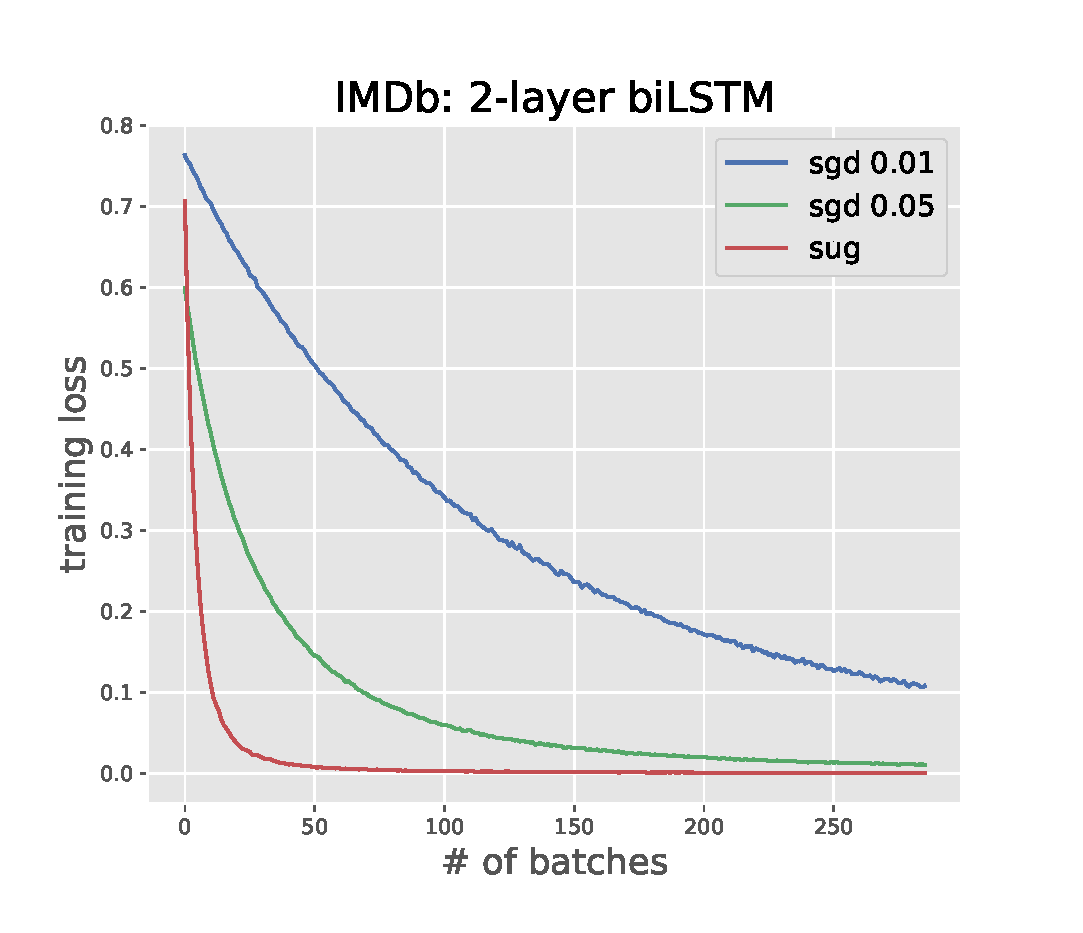
\includegraphics[width=1\textwidth]{figures/imdb_bilstm_bt.eps}
	\end{center}
\end{minipage}
\begin{minipage}{0.5\textwidth}
	\begin{center}
		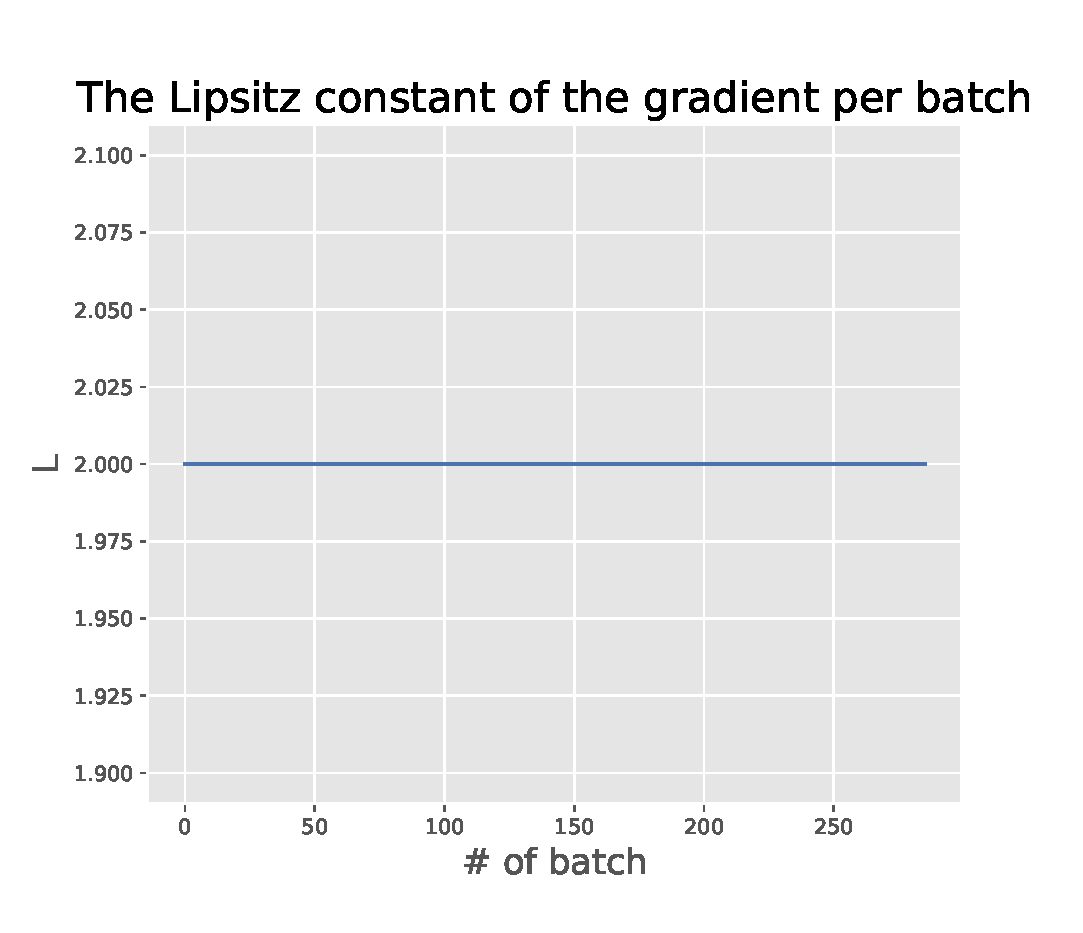
\includegraphics[width=1\textwidth]{figures/imdb_lstm_L.eps}
	\end{center}
\end{minipage}
\medskip
\hrule\medskip
\Head{Further actions}\\
Although the method seems to work well especialy on complex models, still there are several circumstances that are to be overcomed. Doubled time of iteration comparing to the other methods is among them. Besides to maintain the process of optimization stable and avoid undesirable behaviour of the algorithm it was decided to forbid the Lipsitz constant become smaller than 2. That is perhaps an extra constraint not required in theory, so it would be preferable to discard this limit. Still the example with IMDb dataset shows that the method may help significantly decrease the number of optimization steps; the hypothesis is that the solver outperforms others when used to learn complex models. Further it is planned to check this idea on modern neural networks.

\medskip
\hrule\medskip
\Head{Links}\\
\href{https://nbviewer.jupyter.org/github/sverdoot/optimizer-SUG-torch/tree/master/}{You can watch the project here}


\end{textblock}

\end{document}